\documentclass{article}

%%%%%%%%%%%%%%% LIBRERIAS %%%%%%%%%%%%%%%%%%%%%
\usepackage[thinc]{esdiff}
\usepackage{amsmath,amssymb}
\usepackage{caption}
\usepackage{titlesec}
\usepackage{titletoc}
\usepackage{graphicx}
\IfFileExists{spanish.ldf}
  {\usepackage[spanish,es-tabla]{babel}}
  {\usepackage[provide=*,spanish]{babel}}
\usepackage{hyperref}
\usepackage{float}
\usepackage[table]{xcolor}
\usepackage{circuitikz}
\usepackage[left=2cm, right=2cm, top=2cm, bottom=2cm, footskip=1cm]{geometry}
\usepackage{subfiles}
\usepackage{subcaption}
\usepackage{booktabs}
\usepackage{grffile}
\usepackage{comment}
\usepackage{pgfplots}
\pgfplotsset{compat=1.18}
\usepackage{pgfplotstable}
\usepgfplotslibrary{groupplots}

\usepackage{array}
\usepackage{longtable}
\usepackage{tabularx}
\usepackage{enumitem}
\usepackage{setspace}
\usepackage{fancyhdr}
\usetikzlibrary{babel,arrows.meta,calc,positioning}

%%%%%%%%%%%%%%%%%%% VARIABLES %%%%%%%%%%%%%%%%%%%%
\newcommand{\Facultad}{Instituto Tecnológico \\de\\ Buenos Aires}
\newcommand{\TPn}{Trabajo Práctico N° 1}
\newcommand{\TPtema}{Experimento de Millikan}
\graphicspath{{imagenes/}}

%%%%%%%%%%%%%%%%%% FORMATO TÍTULO Y NUMERACIÓN %%%%%%%%%%%%%%%%%%%
\renewcommand{\thesection}{\arabic{section}.}
\renewcommand{\thesubsection}{\thesection\arabic{subsection}}
\renewcommand{\thesubsubsection}{$\alph{subsubsection})$}
\setcounter{secnumdepth}{3}

\titleformat{\section}{\Large\bfseries}{\thesection}{1em}{}
\titleformat{\subsection}{\large\bfseries}{\thesubsection}{0.5em}{}
\titleformat{\subsubsection}{\large\bfseries}{\thesubsubsection}{0.5em}{}

%%%%%%%%%%%%%%% SOPORTE DEL CUERPO DEL INFORME %%%%%%%%%%%%%%%%%%%%%
\definecolor{azulencabezado}{HTML}{163A5F}
\definecolor{azulclaro}{HTML}{EAF2F8}
\definecolor{grislinea}{HTML}{D9D9D9}
\definecolor{grispendiente}{HTML}{5C5C5C}

\newcommand{\pendiente}[1]{\textcolor{grispendiente}{\textit{[#1]}}}
\newcolumntype{Y}{>{\raggedright\arraybackslash}X}
\newcolumntype{C}[1]{>{\centering\arraybackslash}p{#1}}
\newcolumntype{L}[1]{>{\raggedright\arraybackslash}p{#1}}

\hypersetup{
  hidelinks,
  pdftitle={Informe del experimento de Millikan},
  pdfsubject={Laboratorio de Física IV},
  pdfkeywords={Millikan, carga elemental, laboratorio, Física IV}
}

\makeatletter
\providecommand{\ttl@finishall}{}
\makeatother

%%%%%%%%%%%%%%%%%%% ARCHIVO %%%%%%%%%%%%%%%%%%%%%%%%
\begin{document}
\renewcommand{\tablename}{Tabla}
\hypersetup{pageanchor=false}

%%%CARATULA%%%
\begin{titlepage} %creo portada

        \begin{flushleft}
            \centering
            
\includegraphics[width=0.3\textwidth]{Logo_ITBA.png}
        \end{flushleft}

        \centering
            
        {\scshape\LARGE \Facultad \par} 
        \vspace{1cm} 


        {\huge\bfseries \TPn \par}
        \vspace{1.5cm}
        {\Large Laboratorio de Física IV\\ 93.61 \par}
        \vspace{0.5cm}
        {\Large \TPtema \par}
        \vfill 
        {\Large \bfseries Grupo N° 55 \par}
        \vspace{1cm}
        {\large Juan Ignacio Fogolin Lagares \hfill Legajo: 66409  \par}
        {\large Rita Moschini \hfill Legajo: 67026 \par} 
        {\large Agustín Alejandro Montoto \hfill Legajo: 65511\par}
        \vfill
        {\large Fecha de entrega: \today\par}
        \vfill

        \begin{flushleft}
        \renewcommand{\arraystretch}{2.2}
        \begin{tabularx}{\textwidth}{@{}L{8.5cm}Y@{}}
            \toprule
            \textbf{Fecha de aprobación:} & \\
            \midrule
            \textbf{Comentarios y observaciones del docente:} & \\
             & \\
             & \\
            \bottomrule
        \end{tabularx}
        \end{flushleft}

\end{titlepage}

\pagenumbering{gobble}
\tableofcontents 
\newpage

%%%%%%%%%%%%%%%%%%% CUERPO DEL INFORME %%%%%%%%%%%%%%%%%%%%%%%%
\pagenumbering{arabic}
\setcounter{page}{1}
\hypersetup{pageanchor=true}

\setstretch{1.12}
\setlength{\parindent}{0.7cm}
\setlength{\parskip}{0.25em}
\setlength{\arrayrulewidth}{0.45pt}
\setlength{\tabcolsep}{5pt}
\arrayrulecolor{black}
\renewcommand{\arraystretch}{1.28}

\renewcommand{\thesection}{\arabic{section}}
\renewcommand{\thesubsection}{\thesection.\arabic{subsection}}
\setcounter{secnumdepth}{2}

\titleformat{\section}{\Large\bfseries\color{black}}{\thesection}{0.6em}{}
\titleformat{\subsection}{\large\bfseries\color{black}}{\thesubsection}{0.55em}{}
\titlespacing*{\section}{0pt}{1.1em}{0.45em}
\titlespacing*{\subsection}{0pt}{0.9em}{0.35em}

\captionsetup{font={small,it},labelfont=it,justification=centering}
\setlist[itemize]{leftmargin=1.05cm,itemsep=0.18em,topsep=0.25em}
\setlist[enumerate]{leftmargin=1.05cm,itemsep=0.22em,topsep=0.25em}

\pagestyle{fancy}
\fancyhf{}
\fancyhead[L]{\small\itshape Laboratorio de Física IV}
\fancyhead[R]{\small\itshape Instituto Tecnológico de Buenos Aires}
\fancyfoot[C]{\thepage}
\renewcommand{\headrulewidth}{0pt}
\renewcommand{\footrulewidth}{0pt}

\section{Objetivos y resumen}

\subsection{Objetivos}

\begin{itemize}
    \item Determinar la carga de distintas gotas de aceite a partir de su velocidad límite de caída y de la tensión necesaria para mantenerlas en equilibrio dentro de un campo electrostático.
    \item Obtener experimentalmente la carga elemental a partir de la cuantización observada en las cargas calculadas, sin adoptar previamente su valor tabulado.
    \item Analizar la dispersión de las mediciones, estimar sus incertidumbres y reconocer las principales fuentes de error del procedimiento.
\end{itemize}

\subsection{Resumen}

La cuantización de la carga eléctrica es uno de los resultados fundamentales de la física moderna, y el experimento de Millikan permite verificarla experimentalmente sin necesidad de conocer a priori el valor de la carga elemental. Se estudió el movimiento de gotas de aceite cargadas entre las placas paralelas de una celda de Millikan. Para cada una de doce observaciones se ajustó la diferencia de potencial hasta mantener una gota en reposo y se registró la tensión de equilibrio. Luego se anuló el campo eléctrico y se midió el tiempo empleado por la gota para atravesar seis divisiones del retículo. A partir de la velocidad límite se calculó el radio de cada gota mediante la ley de Stokes; con ese radio y la tensión de equilibrio se obtuvo su carga. Finalmente, la carga elemental se determinó buscando el mínimo de una función que mide cuánto se apartan las cargas observadas de múltiplos enteros de un mismo valor.

\textbf{Resultado principal:} Se obtuvo experimentalmente un valor representativo de la carga elemental que resulta $e_{\mathrm{exp}} = (1,378 \pm 0,07) \times 10^{-19}$ C y que conlleva una incertidumbre relativa porcentual del 5,08$\%$.

\section{Introducción teórica}

El experimento se basa en la dinámica de una gota de aceite electrizada. En ausencia de campo eléctrico actúan el peso, el empuje del aire y la fuerza viscosa. Si la gota posee carga y se encuentra entre las placas de un capacitor, también actúa una fuerza eléctrica cuya dirección depende del signo de la carga y de la polaridad aplicada.

\subsection{Caída en un fluido viscoso}

Para una gota esférica de masa $m$, volumen $\Omega$ y densidad $\rho$, el peso aparente $W$ resulta de combinar el peso $P$ con el empuje $Q$ del aire de densidad $\sigma$.

\begin{equation}
P=mg,\qquad Q=-\sigma\Omega g,\qquad W=P+Q=(m-\sigma\Omega)g
\end{equation}

Cuando la gota se desplaza en aire con velocidad $v$, la ley de Stokes describe la fuerza viscosa como

\begin{equation}
F_v=-6\pi\eta a\,v
\end{equation}

donde $\eta$ es la viscosidad dinámica del aire y $a$ es el radio de la gota. Después de un recorrido muy corto, la gota alcanza la velocidad límite $v_L$ y la fuerza neta se anula. El balance vertical queda

\begin{equation}
\frac{4}{3}\pi a^3(\rho-\sigma)g-6\pi\eta a\,v_L=0
\end{equation}

y permite obtener el radio sin observarlo directamente.

\begin{equation}
a=\sqrt{\frac{9\eta v_L}{2(\rho-\sigma)g}}
\end{equation}

\subsection{Equilibrio en el campo electrostático}

Entre placas paralelas separadas una distancia $d$, una diferencia de potencial $V$ produce un campo aproximadamente uniforme. La fuerza eléctrica sobre una gota de carga $q$ es

\begin{equation}
E=\frac{V}{d},\qquad F_e=qE=\frac{qV}{d}
\end{equation}

Al variar $V$ hasta que la gota queda suspendida, su velocidad es nula y no existe fuerza viscosa. La fuerza eléctrica equilibra el peso aparente.

\begin{equation}
\frac{qV}{d}=\frac{4}{3}\pi a^3(\rho-\sigma)g
\end{equation}

Por lo tanto, la carga de cada gota se calcula con

\begin{equation}
q=\frac{4\pi a^3(\rho-\sigma)gd}{3V}
\end{equation}

\subsection{Cuantización de la carga}

Si la carga eléctrica está cuantizada, las cargas $q_i$ obtenidas para diferentes gotas deben aproximarse a múltiplos enteros de una cantidad común $e$. El análisis no debe partir del valor tabulado de $e$: primero se busca el valor que mejor explica el conjunto experimental y recién después se lo compara con una referencia.

\section{Instrumentos y elementos empleados}

El montaje estuvo formado por los siguientes elementos. Los modelos y resoluciones deben completarse con la información del equipo utilizado durante la práctica.

\begin{longtable}{@{}L{3.1cm}L{5.2cm}L{4.6cm}@{}}
    \caption{Instrumentos y elementos del montaje experimental.}\\
    \toprule
    \textbf{Elemento} & \textbf{Función} & \textbf{Especificación relevante} \\
    \midrule
    \endfirsthead
    \toprule
    \textbf{Elemento} & \textbf{Función} & \textbf{Especificación relevante} \\
    \midrule
    \endhead
    \bottomrule
    \endfoot
    Celda de Millikan & Contiene las placas paralelas, el orificio de ingreso y el sistema de iluminación. & $d=5$ mm según la guía \\
    Microscopio con retículo & Permite seleccionar una gota y medir su desplazamiento vertical. & 4,8 divisiones $=2,00$ mm \\
    Fuente regulable de alta tensión & Genera la diferencia de potencial entre las placas. & 0 a 300 V aprox. \\
    Tester o multímetro & Controla la tensión aplicada a la celda. & Resolución: $\pm$3 V \\
    Llave selectora & Conecta, desconecta o invierte la polaridad del campo. & Posiciones utilizadas: campo y neutro \\
    Cronómetro & Mide el tiempo de caída sobre seis divisiones. & Resolución: $\pm$0,01 s \\
    Atomizador con aceite & Produce gotas pequeñas, algunas cargadas por fricción. & Aceite de densidad típica 0,817 g/mL \\
\end{longtable}

\begin{figure}[H]
\centering
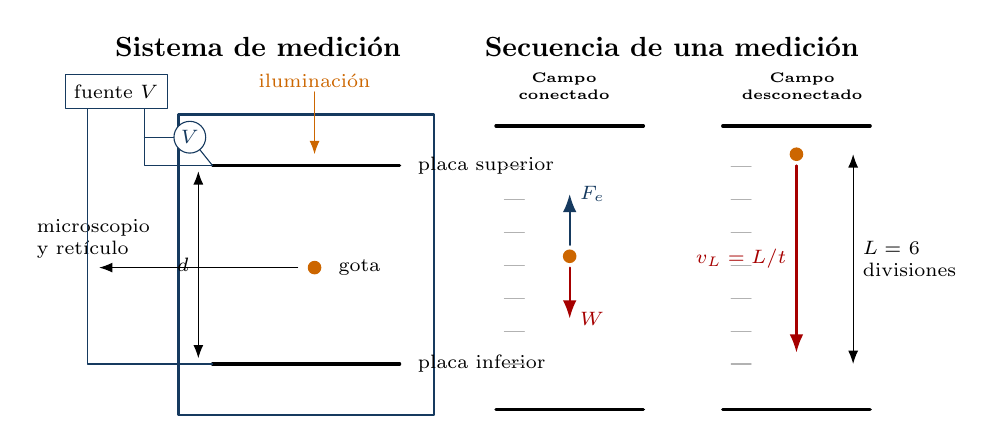
\begin{tikzpicture}[x=0.72cm,y=0.72cm,>=Latex,line cap=round,line join=round]
    \node[font=\bfseries] at (3.5,7.6) {Sistema de medición};
    \draw[azulencabezado,thick] (2.1,1.1) rectangle (6.6,6.4);
    \draw[very thick] (2.7,5.5)--(6.0,5.5);
    \draw[very thick] (2.7,2.0)--(6.0,2.0);
    \node[anchor=west,font=\scriptsize] at (6.15,5.5) {placa superior};
    \node[anchor=west,font=\scriptsize] at (6.15,2.0) {placa inferior};
    \draw[<->] (2.45,2.1)--node[left,font=\scriptsize] {$d$}(2.45,5.4);
    \fill[orange!80!black] (4.5,3.7) circle (0.12);
    \node[anchor=west,font=\scriptsize] at (4.75,3.7) {gota};
    \draw[->] (4.2,3.7)--(0.7,3.7);
    \node[align=left,font=\scriptsize] at (0.6,4.2) {microscopio\\y retículo};
    \draw[orange!80!black,->] (4.5,6.8)--(4.5,5.7);
    \node[orange!80!black,font=\scriptsize] at (4.5,7.0) {iluminación};
    \draw[azulencabezado] (2.7,5.5)--(1.5,5.5)--(1.5,6.5);
    \draw[azulencabezado] (2.7,2.0)--(0.5,2.0)--(0.5,6.5);
    \draw[azulencabezado] (0.1,6.5) rectangle (1.9,7.1);
    \node[font=\scriptsize] at (1.0,6.8) {fuente $V$};
    \draw[azulencabezado] (1.5,6.0)--(2.3,6.0);
    \draw[azulencabezado] (2.7,5.5)--(2.3,6.0);
    \draw[azulencabezado,fill=white] (2.3,6.0) circle (0.28);
    \node[azulencabezado,font=\scriptsize] at (2.3,6.0) {$V$};

    \node[font=\bfseries] at (10.8,7.6) {Secuencia de una medición};
    \node[font=\tiny\bfseries,align=center] at (8.9,6.9) {Campo\\conectado};
    \node[font=\tiny\bfseries,align=center] at (13.1,6.9) {Campo\\desconectado};
    \foreach \x in {7.7,11.7}{
        \draw[very thick] (\x,6.2)--++(2.6,0);
        \draw[very thick] (\x,1.2)--++(2.6,0);
        \foreach \k in {0,...,6}{\draw[gray!60] (\x+0.15,2.0+0.58*\k)--++(0.35,0);}
    }
    \fill[orange!80!black] (9.0,3.9) circle (0.12);
    \draw[azulencabezado,->,thick] (9.0,4.1)--(9.0,5.0) node[right,font=\scriptsize] {$F_e$};
    \draw[red!65!black,->,thick] (9.0,3.7)--(9.0,2.8) node[right,font=\scriptsize] {$W$};
    \fill[orange!80!black] (13.0,5.7) circle (0.12);
    \draw[red!65!black,->,thick] (13.0,5.5)--(13.0,2.2) node[midway,left,font=\scriptsize] {$v_L=L/t$};
    \draw[<->] (14.0,2.0)--node[right,font=\scriptsize,align=left] {$L=$ 6\\divisiones}(14.0,5.7);
\end{tikzpicture}
\caption{Esquema del montaje y de las dos etapas de cada medición.}
\end{figure}

\section{Procedimiento experimental}

\begin{enumerate}
    \item Se ajustó el ocular del microscopio hasta observar con nitidez el retículo y se verificaron la iluminación, la polaridad y la variación de la fuente.
    \item Con la llave en posición neutra y la tensión en cero, se introdujo una pequeña cantidad de aceite atomizado en la celda.
    \item Se conectó el campo eléctrico y se aumentó lentamente la tensión hasta identificar una gota cuya velocidad pudiera reducirse a cero.
    \item Se ajustó finamente la diferencia de potencial hasta mantener la gota en reposo y se registró la tensión de equilibrio $V$.
    \item Se desplazó la gota hasta la zona inicial del retículo, se llevó la llave a la posición neutra y se inició el cronometraje.
    \item Se midió el tiempo $t$ empleado por la gota para recorrer seis divisiones. Durante ese tramo se consideró que la gota caía con velocidad terminal constante.
    \item El procedimiento se repitió hasta reunir doce pares de datos formados por la tensión de equilibrio y el tiempo de caída.
\end{enumerate}

\section{Datos obtenidos y cálculos}

\subsection{Datos experimentales}

La distancia recorrida al atravesar seis divisiones se obtiene de la calibración indicada en la guía.

\begin{equation}
L=6\left(\frac{2,00\,\mathrm{mm}}{4,8}\right)=2,50\,\mathrm{mm},\qquad v_L=\frac{L}{t}
\end{equation}

Si el retículo o la cantidad efectiva de divisiones utilizados fueron diferentes, debe reemplazarse $L$ por el valor correspondiente antes de procesar las mediciones.

\begin{table}[H]
\centering
\small
\caption{Datos primarios de las doce observaciones.}
\begin{tabular}{@{}C{1.8cm}C{2.9cm}C{3.3cm}@{}}
    \toprule
    \textbf{Medición} & \textbf{$V$ equilibrio (V)} & \textbf{$t$ para 6 div. (s)} \\
    \midrule
    1  & 10  & 56,65 \\
    2  & 109 & 69,13 \\
    3  & 61  & 28 \\
    4  & 5   & 114,75 \\
    5  & 50  & 6,4 \\
    6  & 79  & 28,7 \\
    7  & 173 & 39,66 \\
    8  & 53  & 10,6 \\
    9  & 56  & 10,28 \\
    10 & 38  & 6,9 \\
    11 & 61  & 14,67 \\
    12 & 49  & 3,67 \\
    \bottomrule
\end{tabular}
\end{table}

\subsection{Constantes y parámetros adoptados}

\begin{table}[H]
\centering
\small
\caption{Constantes de cálculo.}
\begin{tabular}{@{}L{3.8cm}C{1.7cm}L{3.7cm}L{4.0cm}@{}}
    \toprule
    \textbf{Magnitud} & \textbf{Símbolo} & \textbf{Valor utilizado} & \textbf{Observación} \\
    \midrule
    Viscosidad del aire & $\eta$ & $1,83\times10^{-5}$ N s/m$^2$ & Valor típico a 23 $^{\circ}$C \\
    Densidad del aceite & $\rho$ & 817 kg/m$^3$ & Equivale a 0,817 g/mL \\
    Densidad del aire & $\sigma$ & 1,0 kg/m$^3$ & Equivale a 0,001 g/mL \\
    Separación entre placas & $d$ & $5,00\times10^{-3}$ m & Valor típico de la celda \\
    Aceleración gravitatoria & $g$ & 9,81 m/s$^2$ & Valor adoptado \\
    Distancia sobre el retículo & $L$ & $2,50\times10^{-3}$ m & Seis divisiones \\
    \bottomrule
\end{tabular}
\end{table}

\subsection{Cálculo de la velocidad el radio y la carga}

Para cada observación se calcula $v_L=L/t$, se reemplaza en la ecuación 4 para obtener $a$ y luego se emplea la ecuación 7 para determinar $q$. También puede utilizarse la expresión combinada

\begin{equation}
q=\frac{4\pi d}{3V}\left(\frac{9\eta L}{2t}\right)^{3/2}\frac{1}{\sqrt{(\rho-\sigma)g}}
\end{equation}

\begin{table}[H]
\centering
\small
\caption{Resultados intermedios y carga calculada para cada observación.}
\begin{tabular}{@{}C{1.2cm}C{2.5cm}C{2.3cm}C{2.6cm}C{2.6cm}@{}}
    \toprule
    \textbf{Med.} & \textbf{$v_L$ (m/s)} & \textbf{$a$ (m)} & \textbf{$q$ (C)} & \textbf{$\Delta q$ (C)} \\
    \midrule
    1 & [\quad] & [\quad] & [\quad] & [\quad] \\
    2 & [\quad] & [\quad] & [\quad] & [\quad] \\
    3 & [\quad] & [\quad] & [\quad] & [\quad] \\
    4 & [\quad] & [\quad] & [\quad] & [\quad] \\
    5 & [\quad] & [\quad] & [\quad] & [\quad] \\
    6 & [\quad] & [\quad] & [\quad] & [\quad] \\
    7 & [\quad] & [\quad] & [\quad] & [\quad] \\
    8 & [\quad] & [\quad] & [\quad] & [\quad] \\
    9 & [\quad] & [\quad] & [\quad] & [\quad] \\
    10 & [\quad] & [\quad] & [\quad] & [\quad] \\
    11 & [\quad] & [\quad] & [\quad] & [\quad] \\
    12 & [\quad] & [\quad] & [\quad] & [\quad] \\
    \bottomrule
\end{tabular}
\end{table}

\textbf{Ejemplo de cálculo con la medición 1:} \pendiente{SUSTITUIR $V_1$ Y $t_1$ EN LAS ECUACIONES 8, 4 Y 7, CONSERVANDO UNIDADES DEL SI}

\section{Discusión y cálculo de errores}

\subsection{Incertidumbres de las magnitudes medidas}

Las incertidumbres directamente asociadas al procedimiento provienen principalmente de la lectura de la tensión, la resolución y el tiempo de reacción del cronometraje, y la determinación de la distancia recorrida sobre el retículo. Las incertidumbres de $d$ y de las constantes deben incluirse si sus valores fueron medidos o informados con tolerancia.

Para variables independientes, la propagación de la velocidad límite es

\begin{equation}
\frac{\Delta v_L}{v_L}=\sqrt{\left(\frac{\Delta L}{L}\right)^2+\left(\frac{\Delta t}{t}\right)^2}
\end{equation}

Si $q$ se calcula mediante la ecuación 9 y se consideran exactas las constantes indicadas por la cátedra, su incertidumbre relativa puede estimarse con

\begin{equation}
\frac{\Delta q}{q}=\sqrt{\left(\frac{\Delta d}{d}\right)^2+\left(\frac{\Delta V}{V}\right)^2+\left(\frac{3\Delta L}{2L}\right)^2+\left(\frac{3\Delta t}{2t}\right)^2}
\end{equation}

Si $d$ también se adopta como exacta, se elimina su término. Cuando la cátedra solicite incluir incertidumbres de $\eta$, $\rho$, $\sigma$ o $g$, deben agregarse mediante propagación desde la ecuación 9. No debe contarse dos veces una misma contribución: si se propaga desde la expresión combinada, no se agrega además una incertidumbre de $a$ calculada con las mismas variables.

\subsection{Fuentes de error y dispersión}
\enlargethispage{\baselineskip}

\begin{itemize}
    \item Criterio visual para decidir que la gota estaba inmóvil. Un pequeño movimiento residual modifica la tensión asignada al equilibrio.
    \item Tiempo de reacción al iniciar y detener el cronómetro y dificultad para identificar el cruce exacto de las marcas del retículo.
    \item Pérdida de foco, movimiento fuera del plano observado o selección accidental de otra gota durante la secuencia.
    \item Fluctuaciones de la tensión y resolución limitada del tester y de la fuente.
    \item Diferencias entre la temperatura real y la temperatura asociada a la viscosidad tabulada, junto con las aproximaciones de gota esférica, campo uniforme y validez de la ley de Stokes.
\end{itemize}

\textbf{Observaciones específicas de la práctica:} 

Durante la práctica se dificultó la visualización de las gotas debido a la iluminación, el contraste, su reducido
 tamaño y la alta concentración de estas. Esto ocurrió a distintos niveles de gravedad dependiendo del 
estudiante y afecta directamente la incertidumbre de las mediciones.

\section{Determinación de la carga elemental}

Para cada valor candidato $e$ se calcula el entero $n_i$ más próximo a $q_i/e$ y se evalúa la suma de los apartamientos cuadráticos

\begin{equation}
f(e)=\sum_i\left(\frac{q_i}{e}-n_i\right)^2,\qquad n_i=\operatorname{round}\!\left(\frac{q_i}{e}\right)
\end{equation}

Se recorre un intervalo de valores candidatos, por ejemplo desde $1,0\times10^{-19}$ C hasta $1,7\times10^{-19}$ C con incrementos de $0,001\times10^{-19}$ C, o el intervalo que confirme el docente. El mínimo de $f(e)$ proporciona la estimación experimental inicial. La función debe graficarse con $e$ en el eje horizontal y $f(e)$ en el eje vertical.

\begin{figure}[H]
    \centering
    \pendiente{INSERTAR GRÁFICO DE $f(e)$ CON EL MÍNIMO IDENTIFICADO}
    \caption{Función de ajuste empleada para determinar la carga elemental.}
\end{figure}

Para estimar el efecto de las incertidumbres se repite la minimización usando los extremos $q_i+\Delta q_i$ y $q_i-\Delta q_i$.

\begin{equation}
f_{+}(e)=\sum_i\left(\frac{q_i+\Delta q_i}{e}-n_i\right)^2,\qquad
f_{-}(e)=\sum_i\left(\frac{q_i-\Delta q_i}{e}-n_i\right)^2
\end{equation}

Si $e_+$ y $e_-$ son las posiciones de los dos mínimos, el resultado representativo y su error absoluto se expresan como

\begin{equation}
e_{\mathrm{exp}}=\frac{e_++e_-}{2},\qquad
\Delta e=\frac{\left|e_+-e_-\right|}{2}
\end{equation}

\begin{table}[H]
\centering
\small
\caption{Síntesis del ajuste y resultado final.}
\begin{tabularx}{\textwidth}{@{}>{\bfseries}L{5.5cm}Y@{}}
    \toprule
    Mínimo con $q_i$ & $e_0=$ [COMPLETAR] C \\
    Mínimo con $q_i+\Delta q_i$ & $e_+=$ [COMPLETAR] C \\
    Mínimo con $q_i-\Delta q_i$ & $e_-=$ [COMPLETAR] C \\
    \midrule
    Resultado experimental & $e_{\mathrm{exp}}=$ ([COMPLETAR] $\pm$ [COMPLETAR]) C \\
    Valor de referencia & $e_{\mathrm{ref}}=$ [COMPLETAR DESPUÉS DEL AJUSTE] C \\
    \bottomrule
\end{tabularx}
\end{table}

La comparación con el valor de referencia se realiza solamente después de obtener $e_{\mathrm{exp}}$.

\begin{equation}
\varepsilon_r=\frac{\left|e_{\mathrm{exp}}-e_{\mathrm{ref}}\right|}{e_{\mathrm{ref}}}\times100\%
\end{equation}

\section{Análisis de los resultados obtenidos}

\textbf{Interpretación global:} \pendiente{RELACIONAR EL MÍNIMO DE $f(e)$, LOS ENTEROS $n_i$ Y EL CARÁCTER CUANTIZADO DE LA CARGA}

\section{Conclusiones}

Mediante la combinación de la caída a velocidad terminal y el equilibrio electrostático se 
obtuvo la carga de cada gota sin medir directamente su masa ni su radio. El valor de la carga 
elemental deducido del conjunto fue $e_{\mathrm{exp}} = (1,378 \pm 0,07) \times 10^{-19}$ C. 
La diferencia relativa respecto del valor de referencia fue del 14$\%$. \pendiente{INDICAR SI EL RESULTADO FUE COMPATIBLE Y CUÁL FUE LA LIMITACIÓN EXPERIMENTAL DOMINANTE}

\end{document}
